\chapter{Asking Billionaires If They Believe In God!}

This lecture from School of Hard Knocks, in a companion-note draft curated by LazyingArt LLC, begins in an unusual way. We do not begin with doctrine, nor even with a clean thesis. We begin with money numbers thrown at us in rapid succession: almost half a billion, nearly two billion, billions across a portfolio, millionaire at twenty-two. Only then does the host ask the governing question: do the people at the top believe their success came from hard work alone or from something greater? The mathematics here is therefore modest but not trivial. It lies in keeping categories distinct, tracing how scale is introduced, and seeing how the lecture repeatedly moves from amount to mechanism and from mechanism to meaning.

\begin{remark}
No validated board images or diagram screenshots survive for this lecture. Every equation and schematic below is transcript-driven or cautiously reconstructed from the spoken sequence rather than transcribed from the screen.
\end{remark}

\section{Scale before belief}

The teaser montage is a compressed catalogue of outcomes. A son's father sold for almost half a billion. A couple sold to PepsiCo for nearly \$2 billion. A veteran investor says that across his companies the scale is in the billions. Tim Tebow reports millionaire status at about twenty-two. The host deliberately lets these numbers accumulate before he names the theological experiment. The effect is simple: belief is made to answer to visible worldly scale.

To keep the lecture readable, we should distinguish several kinds of number at once. An annual earning is not the same as a company sale value; a sale value is not the same as the owner's personal proceeds; an aggregate portfolio scale is not the same as a single-company result. Much of the chapter's discipline lies in not letting these categories collapse.

\begin{definition}
We write \(Y\) for annual earnings or salary, \(V_{\text{sale}}\) for the sale value of a company, \(s\) for an ownership share, and \(W_{\text{gross exit}}=sV_{\text{sale}}\) for the implied gross value of that stake. When the lecture speaks loosely, the notes will keep these objects separate.
\end{definition}

After the teaser, the host resets the scene in Austin. He reports more than ten billionaires living there, calls it a top-ten American city for billionaire residents, and says the millionaire count has doubled over the last decade. These claims are not introduced as census tables; they are introduced as field conditions. Austin is not merely a backdrop. It is the chosen search space in which the host expects repeated encounters with wealth.

\begin{align}
B_{\text{Austin}} &> 10,\\
\operatorname{rank}_{\text{billionaire cities}}(\text{Austin}) &\le 10,\\
M_{\text{Austin, now}} &\approx 2\,M_{\text{Austin, decade ago}}.
\end{align}

The host immediately tests that field and encounters refusal. People keep walking. They do not stop long enough to tell a complete story. This matters because the lecture is not built in a studio. It is built in the friction between a direct question and the limited time a stranger will grant.

\subsection{Question \& Answer}

Why begin with wealth figures before the God question? Because in this lecture belief is not treated as a free-floating opinion. It is tested against public measures of success. The numbers come first so that the later claims about faith, purpose, and providence are heard against exits, salaries, and business scale rather than in abstraction.

\section{The first serious witness: portfolio scale and purpose}

The first substantial interview comes from a veteran investor. The initial answers are business-like: critical technology companies, veterans on leadership teams, leadership, resilience, and purpose. Here the lecture is careful. It does not yet say that wealth is explained by faith. It says first that early-stage building is hard and that one needs a reason to continue.

That logic can be written in a deliberately limited way. The investor says he has \(120\) companies in his personal portfolio and that the revenue scale across the board is in the billions. The useful compression is therefore an aggregation, not a valuation theorem.

\begin{equation}
n_{\text{portfolio}} = 120, \qquad
R_{\text{portfolio}} = \sum_{i=1}^{120} R_i, \qquad
R_{\text{portfolio}} \sim \mathcal{O}(10^9).
\end{equation}

The key point is not the exact sum. The key point is that the interviewee speaks in aggregate business scale while the host keeps tightening the question toward interior stability: Do you ever doubt yourself? How did you get over that? The lecture's first serious answer to that tightening is biography. The investor is a first-generation immigrant. His family came with nothing. He describes education, military service, and responsibility. The veteran fund is not described as a hobby or an optimization. It is described as duty.

\subsection{Question \& Answer}

What stabilizes an entrepreneur under doubt? This interview answers: not certainty, and not the absence of fear, but purpose. The chain runs from leadership and resilience to responsibility, and from responsibility to the conviction that one's work is what one is here to do. The segment's compact slogan is therefore not triumphal but structural: you cannot fail when you know why you are here.

\section{Wrestling, reading, and modern-day alchemy}

Only after the investor has grounded himself in responsibility does the host ask the explicit faith question. The answer is unhesitating, but the explanation is not simplistic. The interviewee says that he grows deeper in faith every day, and then immediately refuses the cheap version of that sentence. Depth is not mere assent. It is wrestling.

This is one of the lecture's strongest conceptual turns. Faith is not described as passive acceptance of everything one hears. It is described as an ongoing questioning that does not dissolve belief but thickens it. The lecture is therefore careful not to oppose doubt and faith as absolute enemies. Instead it treats wrestling as one path by which faith becomes intellectually and existentially serious.

The host then asks about books, and the interview shifts once more. \emph{The Alchemist} becomes the bridge from spirituality back into business. Entrepreneurship is called modern-day alchemy: one takes an idea that does not yet exist in the world and makes it real. The precise garbled word in the transcript is unreliable, but the surrounding meaning is clear. The lecture is now describing business creation as a transformation from thought to object, from intention to institution.

We may compress that move schematically without pretending that the lecture offered a formal equation:
\begin{equation}
\text{idea} + \text{execution} \longrightarrow \text{something real}.
\end{equation}

This is not an algebraic law. It is the chapter's cleanest way to preserve a spoken metaphor that the lecture uses seriously. The investor closes with a three-word ethos, ``do great things,'' and again the argument is not merely motivational. It is tied to mortality, gratitude, and what one wishes to have done before the day ends.

\section{From salary to exit}

The next major interview arrives through an accidental route. A young man says the host is missing the richest guy here, namely his father. The father turns out to be a healthcare founder whose business sold for \$460 million. This segment matters because it gives us the lecture's sharpest wealth mechanism. The interview starts with hardship: South Africa, periods of living in a car, family instability, and then the American dream. But when the host asks for the turning point to financial freedom, the answer is not a vague story about mindset. It is an ownership event.

Before the exit, the founder describes a salary in the rough range of \$100{,}000 to \$120{,}000 while trying to pay for children's opportunities and maintain the household. The lecture then compresses years of effort into a single decisive transition: financial freedom came in one massive check.

\subsection{Question \& Answer}

What was the turning point to financial freedom? In the lecture's own order, it was not gradual salary accumulation. It was the sale of a business for \$460 million, combined with substantial ownership in that business. The contrast is not between work and no work; it is between wage flow and ownership-based liquidity.

We can write that reconstruction carefully:
\begin{align}
Y_{\text{salary}} &\approx \$100{,}000\text{--}\$120{,}000,\\
V_{\text{sale}} &\approx \$460\times 10^6,\\
s &\approx \tfrac12,\\
W_{\text{gross exit}} &\approx sV_{\text{sale}} \approx \$230\times 10^6.
\end{align}

The last line is only a gross ownership estimate. It is not a quoted payout. It ignores taxes, dilution, debt, and transaction structure. But it is still the right mathematical reconstruction of the lecture's point: the category that changed life was not salary but stake.

\paragraph{Worked example.}
The arithmetic is short, but the lecture needs it.
\begin{enumerate}
\item The company sale value is reported as \(V_{\text{sale}} \approx \$460\times 10^6\).
\item The ownership share is reported as \(s \approx \tfrac12\).
\item Multiplying sale value by stake gives an implied gross value of the founder's position.
\item Hence
\[
W_{\text{gross exit}} \approx \tfrac12(\$460\times 10^6) \approx \$230\times 10^6.
\]
\item The explanatory contrast is then
\[
Y_{\text{salary}} \ll W_{\text{gross exit}}.
\]
\end{enumerate}

\begin{figure}
\centering
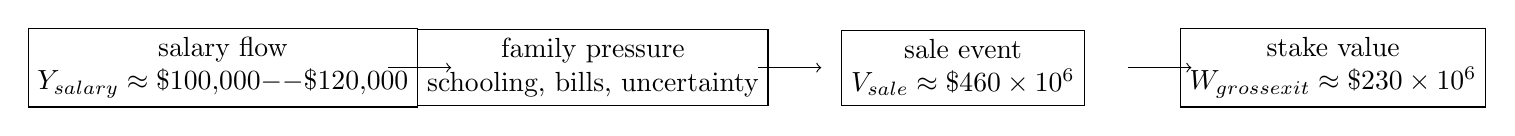
\begin{tikzpicture}[x=1cm,y=1cm]
\node[draw, align=center] at (0,0) (salary) {salary flow\\$Y_{\text{salary}}\approx \$100{,}000\text{--}\$120{,}000$};
\node[draw, align=center] at (4.7,0) (pressure) {family pressure\\schooling, bills, uncertainty};
\node[draw, align=center] at (9.4,0) (sale) {sale event\\$V_{\text{sale}}\approx \$460\times 10^6$};
\node[draw, align=center] at (14.1,0) (stake) {stake value\\$W_{\text{gross exit}}\approx \$230\times 10^6$};
\draw[->] (2.1,0) -- (2.9,0);
\draw[->] (6.8,0) -- (7.6,0);
\draw[->] (11.5,0) -- (12.3,0);
\end{tikzpicture}
\caption{A transcript-derived schematic of the lecture's clearest wealth mechanism: incremental salary on one side, ownership and liquidation on the other. This is a note-writing aid, not a figure shown in the video.}
\end{figure}

The surrounding interview keeps the arithmetic from becoming merely financial. The founder says he believes in God, credits Jesus Christ, and speaks of divine favor as a background confidence that allowed him to start and risk. Again, the lecture does not ask us to confuse testimony with proof. It asks us to preserve the causal language the speaker himself uses.

The segment then widens. AI is treated as an unavoidable wave, both exciting and frightening, and the founder insists that healthcare businesses should stand in the middle of it if it can lower cost and help more people. A sponsor interlude follows, built around AI-assisted note capture. This belongs to the transcript order and should remain visible as an interruption, though it should not be mistaken for the chapter's central doctrine. The more durable line of thought comes just after: surround yourself with people who stretch you, keep reading, expect rejection, and refuse comfort. The lecture's social arithmetic is not a formula but a direction of movement: the right room is the room in which one is least impressive.

A final line from this segment deserves to be preserved in compressed symbolic form. When the founder says that some investors got \(75X\) on a first investment, he is not giving us a venture theorem. He is giving scale.
\begin{equation}
M_{\text{return}} \approx 75.
\end{equation}

\section{Evidence, mission, and legacy}

The Tim Tebow interview begins, characteristically, with money. He became a millionaire around age twenty-two and reports a best NFL year somewhere between \$5 million and \$10 million. The lecture keeps the category narrow: these are annual earnings and age markers, not a full net-worth statement.

\begin{equation}
A_{\text{millionaire,Tebow}} \approx 22, \qquad
Y_{\text{Tebow}} \in [\$5,\$10]\times 10^6.
\end{equation}

Once again, however, the lecture does not linger on the number. It moves almost immediately to belief. Tebow's answer is more explicitly evidential than the earlier ones: he points to the Bible, the cross, the resurrection, testimony, the transformed boldness of the disciples, and the implausibility, in his view, of saying that nothing created all this. We should preserve the structure of this reasoning without rewriting it as a formal proof. The lecture presents it as compressed public apologetics, not as a deductive theorem.

The next shift is from belief to mission. Tebow says he now works against human trafficking, child exploitation, and child sacrifice, and he gives the numbers not to impress but to convey magnitude. The scale is moral rather than entrepreneurial, but it is still scale.

\begin{equation}
N_{\text{trafficked}} > 50\times 10^6, \qquad
N_{\text{exploited}} > 400\times 10^6.
\end{equation}

The host then asks for life-changing advice, and the interview reaches its cleanest payoff. The greatest tragedy, Tebow says, is to be successful at everything that does not matter. This is the lecture's sharpest inversion of its own premise. We began with large numbers. We are now told that large numbers can be attached to the wrong target.

\subsection{Question \& Answer}

What matters more than success? The lecture answers by narrowing the word \emph{success} until it becomes morally legible. Success in itself is not enough. The serious question is whether success attaches to what matters. Hence the distinction between inheritance, what one leaves for someone, and legacy, what one leaves in someone. The lecture does not reject achievement; it asks achievement to answer for its object.

The host's recap after this segment is important. Tebow is not kept as a celebrity cameo. He is repositioned as a case in which early money is real, but later mission becomes the true measure.

\section{Trust after the \$2 billion sale}

The final substantial interview is with a married couple who sold a company to PepsiCo for roughly \$2 billion. Here too the lecture preserves order carefully: first the sale, then the marriage, then the joint business structure, then the principles that kept wealth from closing the story.

\begin{equation}
V_{\text{Pepsi exit}} \approx \$2\times 10^9, \qquad
t_{\text{marriage}} = 12\ \text{years}, \qquad
n_{\text{children}} = 3.
\end{equation}

The decisive answer in this section is trust. If partners do not trust each other to do what they say they will do, then neither marriage nor business can hold. Purpose then enters again, and in a particularly valuable form. They say plainly that freedom does not equal purpose. This is one of the lecture's cleanest conceptual distinctions, and it deserves to be written with the simplicity the speakers themselves give it.

\begin{equation}
F_{\text{financial freedom}} \neq P_{\text{purpose}}.
\end{equation}

Their post-exit life is therefore not retirement in the ordinary sense. It is freedom of choice about with whom to work and what to build next. The lecture again refuses to let money be the last explanation.

The broke-beginning story adds another layer. Early in the business, with a child, a mortgage, and deep uncertainty, a tax refund arrived almost exactly at the level of the payment due. In the lecture this is narrated as providential reassurance, not as financial theory. But the underlying compression is still useful because it shows how the story is remembered:
\begin{equation}
F_{\text{refund}} \approx M_{\text{mortgage}}.
\end{equation}

The couple then gives the closing growth logic of the lecture. People say they want what others have, but they often do not want the discomfort required to get there. Balance is not rejected absolutely, but entrepreneurial growth is said to be inseparable from uncomfortable moments, embarrassment, and repeated exposure to situations in which one does not yet know what one is doing. The final progression is strikingly clean:
\begin{equation}
\text{embarrassment} \longrightarrow \text{refinement} \longrightarrow \text{clarity} \longrightarrow \text{confidence}.
\end{equation}

\subsection{Question \& Answer}

What keeps freedom from collapsing into purposeless retirement? The lecture answers with a three-part structure: trust, shared purpose, and continued execution. Money may buy options, but it does not choose a goal. Without a common aim, freedom becomes drift; with a common aim, freedom becomes a new phase of work.

The section closes with one more compression, now directed at the next generation. If the world was built by people no smarter than we are, then the bar is not genius but willingness: willingness to work, to risk embarrassment, and to keep moving before confidence arrives.

\section{Summary}

This lecture begins with spectacle, but it is not finally about spectacle. Its numerical spine is clear enough: Austin as a dense search field, a \(120\)-company portfolio, a \$460 million healthcare exit with roughly half ownership, NFL earnings in the \$5--\$10 million range, a \$2 billion sale to PepsiCo, and very large social-mission counts in Tebow's segment. Yet the lecture's real movement is not from small numbers to big numbers. It is from amount to mechanism, and then from mechanism to explanation.

The notes therefore preserve two things at once. First, the concrete business distinctions: salary versus exit, sale value versus ownership, annual earnings versus portfolio scale. Second, the recurring interpretive claim made by the speakers themselves: wealth is repeatedly narrated not as a self-explaining endpoint but as something answered by purpose, faith, mission, trust, and the willingness to endure discomfort. That is the order in which the lecture teaches, and it is the order in which these companion notes should be read.